Instead of discarding the human factor, this experiment aims at testing if the human factor is able to find and synchronize an User Generated Video dataset. The Climbing video dataset \cite{hal-01162603} presents multiple videos filmed by a group during a climbing activity. The automatic technique presented with the dataset presents some limitations making this dataset ideal to test the crowd approach, so we selected part of the dataset (9 videos) to our experiment. The automatic method could identify 23\% of all pairs of videos that temporally overlap, the pairwise alignment score (PAS).

To execute our experiment, we developed the technique described in section~\ref{chunk-sync}, where the crowd member analyse video chunks (5s) pair by pair, identifying if there is relation and the precision of the relation if one exists. This was the chosen solution because requires less effort from the crowdworkers, and more detailed tests are necessary to evaluate the Frame Synchronization one, as a more complex task may compromise the worker activity.

From the known ground-truth we analysed the values resulted from the crowd to evaluate the alignment within a tolerance of 0.5s \cite{hal-01162603}. The comparison with the ground truth resulted in 88\% (PAS) of correct relations among the videos. The nine videos generated 278 chunks of video (a total of 1390 seconds to be synchronized) demanding a total of 1051 contributions. Most of these (99\%) contributions were negative ones, in other words, the crowd worker could not identify synchronization  point. This indicates that most of the crowd effort is being done in discarding synchronization point, and not really finding them.

Figure~\ref{interface} shows an instant where overlapping occurs in videos recorded using 6 different cameras are synchronously presented after the crowd contributions. The other three ones are not shown because in this instant no overlapping was indicated by the crowd. It is possible to notice how heterogeneous are the camera shots. 

\begin{figure}[h]
	\centerline{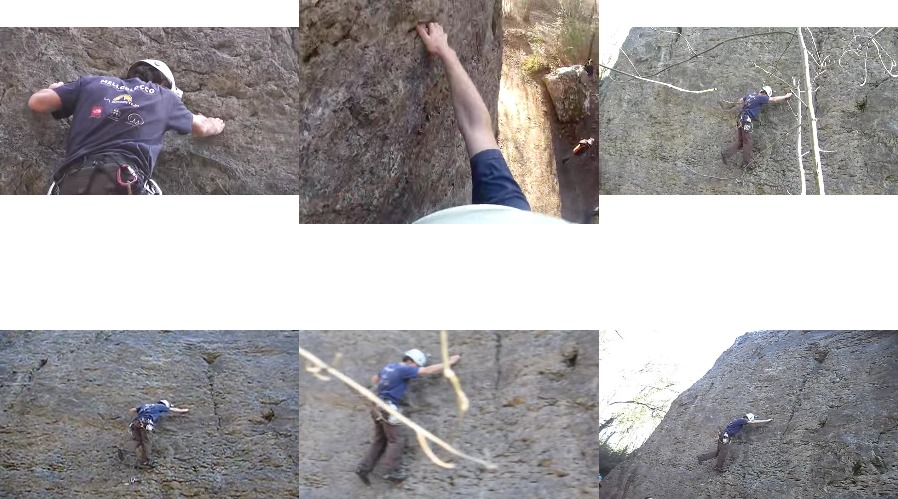
\includegraphics[scale=0.2] {figure/matrix}}
	\caption{Synchronized Video Matrix}
	\label{interface}
\end{figure}